\documentclass[tikz,border=2pt]{standalone}
\usepackage{lmodern}
\usepackage{pgfplots}
\pgfplotsset{compat=1.18,every axis/.append style={
 font=\fontsize{9}{11}\selectfont,tick label style={font=\fontsize{9}{11}\selectfont},
 label style={font=\fontsize{9}{11}\selectfont},title style={font=\fontsize{9}{11}\selectfont},
 axis line style={black!50,line width=.4pt},tick style={black!50},
 axis lines*=left,clip=false,legend style={draw=none,font=\fontsize{9}{11}\selectfont},
 scaled ticks=false}}
\definecolor{accent}{HTML}{365F7D}
\begin{document}
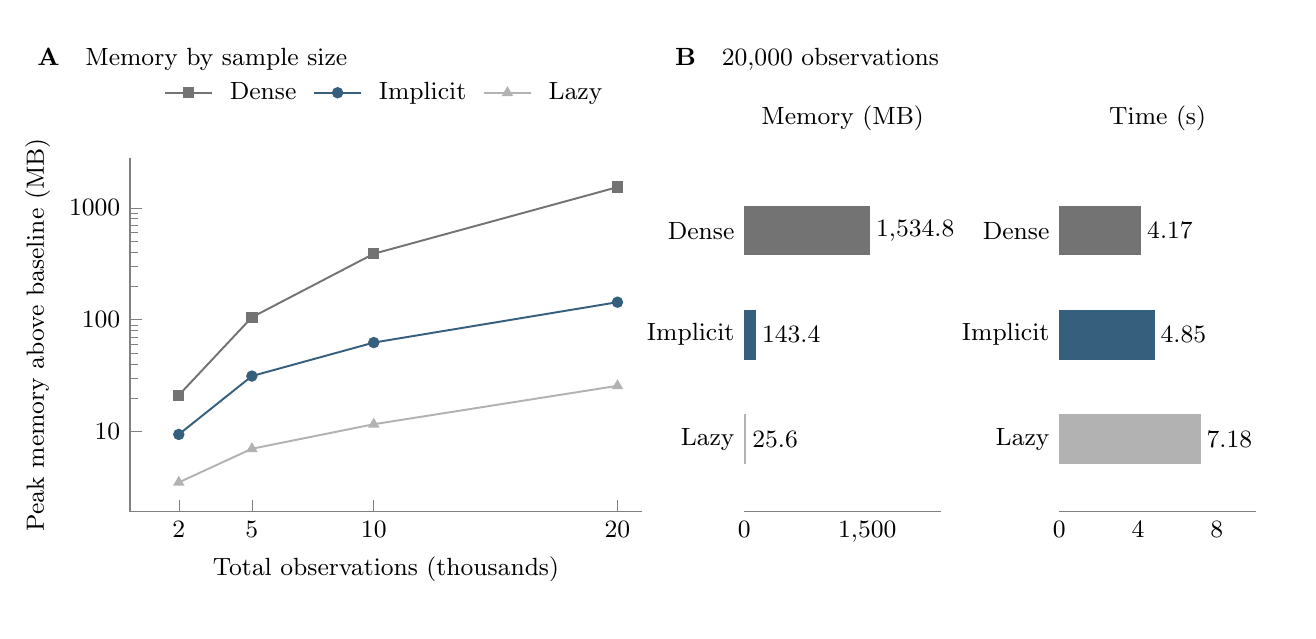
\begin{tikzpicture}[font=\fontsize{9}{11}\selectfont]
\path[use as bounding box] (0,0) rectangle (16,7.4);
\node[anchor=west] at (0,7.0) {\textbf{A}\quad Memory by sample size};
\node[anchor=west] at (8.1,7.0) {\textbf{B}\quad 20,000 observations};
\begin{axis}[at={(1.3cm,1.25cm)},anchor=south west,width=6.5cm,height=4.5cm,
 scale only axis,ymode=log,xmin=0,xmax=21,xtick={2,5,10,20},ytick={10,100,1000},
 yticklabels={10,100,1000},xlabel={Total observations (thousands)},
 ylabel={Peak memory above baseline (MB)},legend columns=3,
 legend style={at={(.5,1.12)},anchor=south,column sep=4pt}]
\addplot[color=black!55,mark=square*,mark size=1.7pt,line width=.7pt] coordinates {(2.0,21.1) (5.0,105.1) (10.0,388.9) (20.0,1534.8)};
\addlegendentry{Dense}
\addplot[color=accent,mark=*,mark size=1.7pt,line width=.7pt] coordinates {(2.0,9.4) (5.0,31.3) (10.0,62.4) (20.0,143.4)};
\addlegendentry{Implicit}
\addplot[color=black!30,mark=triangle*,mark size=1.7pt,line width=.7pt] coordinates {(2.0,3.5) (5.0,7.0) (10.0,11.6) (20.0,25.6)};
\addlegendentry{Lazy}
\end{axis}
\begin{axis}[at={(9.1cm,1.25cm)},anchor=south west,width=2.5cm,height=4.5cm,scale only axis,xbar,bar width=18pt,bar shift=0pt,xmin=0,xmax=2400,ymin=-.7,ymax=2.7,ytick={0,1,2},yticklabels={Lazy,Implicit,Dense},xtick={0,1500},title={Memory (MB)},y axis line style={draw=none},tickwidth=0pt]
\addplot[fill=black!55,draw=none] coordinates {(1534.8,2)};
\node[anchor=west,inner sep=2pt] at (axis cs:1534.8,2){1,534.8};
\addplot[fill=accent,draw=none] coordinates {(143.4,1)};
\node[anchor=west,inner sep=2pt] at (axis cs:143.4,1){143.4};
\addplot[fill=black!30,draw=none] coordinates {(25.6,0)};
\node[anchor=west,inner sep=2pt] at (axis cs:25.6,0){25.6};
\end{axis}
\begin{axis}[at={(13.1cm,1.25cm)},anchor=south west,width=2.5cm,height=4.5cm,scale only axis,xbar,bar width=18pt,bar shift=0pt,xmin=0,xmax=10,ymin=-.7,ymax=2.7,ytick={0,1,2},yticklabels={Lazy,Implicit,Dense},xtick={0,4,8},title={Time (s)},y axis line style={draw=none},tickwidth=0pt]
\addplot[fill=black!55,draw=none] coordinates {(4.165,2)};
\node[anchor=west,inner sep=2pt] at (axis cs:4.165,2){4.17};
\addplot[fill=accent,draw=none] coordinates {(4.845,1)};
\node[anchor=west,inner sep=2pt] at (axis cs:4.845,1){4.85};
\addplot[fill=black!30,draw=none] coordinates {(7.184,0)};
\node[anchor=west,inner sep=2pt] at (axis cs:7.184,0){7.18};
\end{axis}
\end{tikzpicture}
\end{document}
